% !TeX root = ../thesis.tex

\chapter{Fundamentals and Related Work}
\label{sec:fundamentals_related-work}
\section{Overview}
The new era of deep neural networks began in 2012, when Krizhevsky et al. published
their results on the ImageNet Large-scale Visual Recognition Challenge (ILSVRC) 
\cite{krizhevsky_imagenet_2017}. Their deep neural network (DNN) has 5 convonlutional layers followed by 2 fully connected layers, which is approximately higher than the closest competitor based on SIFT\cite{sanchez_high-dimensional_2011}. The classification error rate is 10\%. For DNN, this moment is a huge breakthrough because they proved superior to classic computer vision methods. There are multiple
The factors that contributed to this achievement, such as
Train the network to perform multiple orders of magnitude more powerful hardware
New training algorithms and networks have more training iterations than previously possible
The architecture of convolutional layers, etc.
Since then, many DNN methods for image classification and objects have been developed
Detection. In the next section, we will review these methods. The existing method can be
Divided into two groups: regional proposal method and end-to-end learning method.
The former includes the region proposal step and the proposed DNN classifier
Region, the latter is a DNN, used to obtain the original image and directly output information
Regarding the detected object. 
\subsection{}
\section{Datasets}
\begin{enumerate}
\item\textit{KITTI}


The whole work is mainly based on PointPillars\cite{lang_pointpillars_2019}. It has fast inference speed and relative higher detection accuracy.

For adversarial attack the work is based on KITTI\cite{geiger_vision_2013} dataset. This dataset is proposed relative earlier and famous in autonomous driving field. But it didn't consider adverse weather problem.

For adverse weather simulation, the work is based on DENSE\cite{heinzler_cnn-based_2020} dataset. This work have shown how to use this dataset to segment points with weather class. This dataset have collected the point cloud in chamber with man-made adverse weather, there's also clean point cloud. 

\end{enumerate}
CNN
Convolution
PointNet
Adversarial attacks
\begin{figure}[!htbp]
    \centering
    \subfigure[Logo 1]{
        
\includegraphics[width = \textwidth / 2 ]{Logos/KITLogo_RGB.pdf}
        \label{fig:logo1}
    }
    \hspace{10pt}
     %add desired spacing between images, e. g. ~, \quad, \qquad, \hfill etc.
     %(or a blank line to force the subfigure onto a new line)
    \subfigure[Logo 2]{
        
\includegraphics[width = \textwidth / 2 ]{Logos/KITLogo_RGB.pdf}
        \label{fig:logo2}
    }
    \caption[Short Description for List of Figures]{Long Description for under the figure.}
    \label{fig:logo1and2}
\end{figure}

\section{Evaluation of Adversarial Attacks}
\begin{enumerate}
\item\textit{Intersection over union}

Intersection over union means the similarity of two bounding boxes. It is used to compare detected bounding boxes and ground truth bounding boxes. 2D version is shown here:
\begin{center}
          \(IOU_{b_{1},b_{2}} = \frac{A(b_{1}\cap b_{2})}{A(b_{1}\cup b_{2})} \)
\end{center}
where \(A(\bullet)\) represents Area and b, are bounding boxes. For KITTI\cite{geiger_vision_2013} evaluation there's two criterions, \(IOU\geq0.5\) and \(IOU\geq0.7\) to accept a detection as a correct one.

\item\textit(Average Precision)
Precision is the ratio of detected objects \(TP+FP\), which are detected correctly. It shows how many false positive \(FP\) detections the detectors produces. It is defined as follows
\begin{center}
          \(Precision = \frac{TP}{TP+FP} \)
\end{center}
Recall represents the ratio of the ground truth objects \(TP+FN\), which are detected by the detector. It is defined as 
\begin{center}
          \(Recall = \frac{TP}{TP+FN} \)
\end{center}
Average precision (AP) is used in the KITTI benchmark. It samples the precision/recall curve on 11 places, interpolates it and computes the arithmetic mean. Therefore, this measure gives insight into how the precision/recall curve changes. For details see\cite{everingham_pascal_2010}

\end{enumerate}

\section{FGSM and Its Variants}

\begin{enumerate}
\item \textit{FGSM}

FGSM is shorten for fast gradient sign method\cite{goodfellow_explaining_2015}. It uses sign function with gradients, which get from loss function. As the panda example (Figure 4.1) shows the process of FGSM. The left picture is clean image, the classifier predicts the picture a panda. When perturbation is added to the clean image, even the epsilon value is very small, classification result is totally different, the panda is recognized as a gibbon.
\begin{center}
          \(x_{adv} = x + \epsilon sign(\nabla_{x}J(f(x;\theta),y) \)
\end{center}
\begin{figure}[!htbp]
\centering
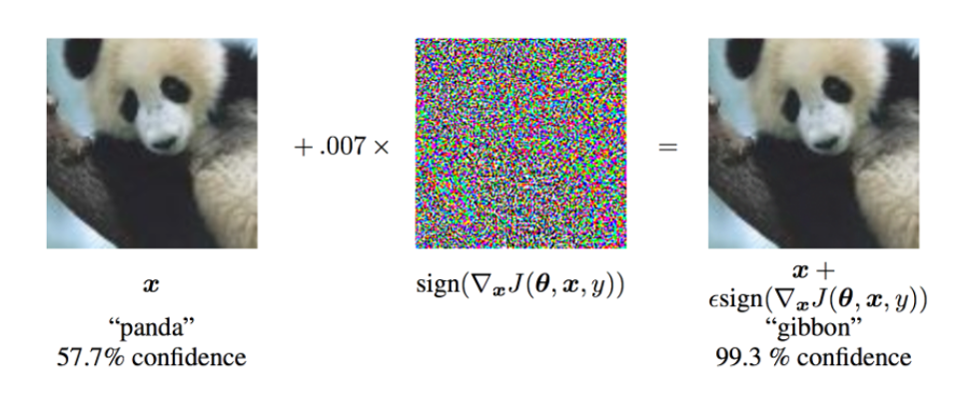
\includegraphics[scale=0.5]{FGSM.png}
\caption{Adversarial attack process of FGSM example}
\label{fig:FGSM}
\end{figure}
\item \textit{IFGSM} 

IFGSM\cite{kurakin_adversarial_2017} is shorten for iterative fast gradient sign method. This method improves FGSM and is also proposed by Goodfellow and his partners. IFGSM applies FGSM multiple times with a small step size. IFGSM performs better than FGSM. When the same clean image is attacked by FGSM and IFGSM with the same total epsilon, the impact of FGSM attack can be easily observed by naked eyes, but attack in IFGSM is imperceptible.
\begin{center}
          \(X_{0}^{adv} = X,  X_{N+1}^{adv}=Clip_{X,\epsilon}{X_{N}^{adv}+\alpha sign(\nabla_{x}J(f(X_{N}^{adv};\theta),y_{true}))} \)
\end{center}
 \item \textit{MIFGSM}
 
 MIFGSM\cite{dong_boosting_2018} is shorten for iterative fast gradient sign method with momentum. This method stabilizes optimization by accumulating gradients at each iteration.
  \begin{center}
          \(x^{*}_{t+1} =x^{*}_{t}+\alpha \frac{g_{t+1}}{\|g_{t+1}\|_{2}},
           g_{t+1} = \mu * g_{t}+\frac{J(X^{*}_{t},y^{*})}{\|\nabla_{x}J(X_{t}^{*},y^{*}\|_{1}} \)
\end{center}
 \item \textit{PGD}
 
 PGD\cite{madry_towards_2019} is shorten for projected gradient descent. Compared with IFGSM, this approach adds random initialization perturbation at the beginning.
 \begin{center}
          \(x^{t+1} =\prod_{x+S}({x^{T}+\alpha sign(\nabla_{x}L(\theta;x;y)))} \)
\end{center}
 
 \item \textit{Fast Gradient Norms}
 
 S in FGSM is sign, which represents  \(L_\infty\) norm. DeepFool\cite{moosavi-dezfooli_deepfool_2016} proposed  \(L_2\) norm to replace sign norm for a better result in image. 
 \begin{center}
          \(x^{*} =x+\sigma\frac{\nabla_{x}J(x,y)}{\|\nabla_{x}J(x,y)\|_{2}} \)
\end{center}
 There's also  \(L_1\) norm as Manhattan metric to replace sign norm. Liu et.al(\cite{liu_adversarial_2019}) proposed a new version of \(L_2\) norm named \(L_2.5\) norm, which is normalized \(L_2\) norm's result. 
 \item \textit{Attack on Different Features} 
 
 LiDAR point clouds have 4 dimensions which are 4 features: \(x\) coordinate, \(y\) coordinate, \(z\) coordinate and intensity \(r\). So there are two different kinds of attack types: one is only attack one feature, which is separately attack \(x\) coordinate, \(y\) coordinate, \(z\) coordinate and intensity \(r\). The other is attack multiple features: \(xyz\) coordinates, and the combination of \(xyz\) coordinates and intensity \(r\). 

\item\textit{Adversarial training}

FGSM-based Adversarial training is an efficient way to defense adversarial attacks of FGSM. The adversarial training of FGSM:
\begin{center}
          \(Loss_{train} = 1/2*(Loss_{original}+Loss_{perturbation}) \)
\end{center}

\end{enumerate}
